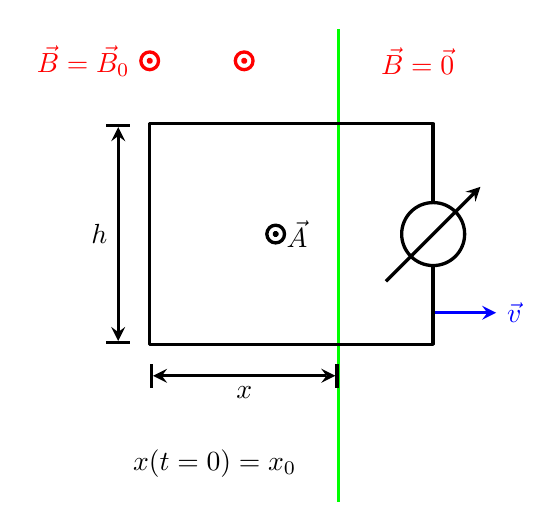
\begin{tikzpicture}[line width = 1.2pt, line join=round,x=1cm,y=1cm,>=stealth, scale = 0.4]
	% Grenzfläche
	\draw [color = green] (0,-5) -- (0,10);
	% Geschwindigkeit
	\draw [color = blue,->] (3,1) -- ++(2,0) node [anchor = west] {$ \vec{v} $};
	% Leiterschleife
	\draw (-6,0) rectangle (3,7);
	\filldraw [fill = white, draw = black] (3,3.5) circle (1);
	\draw [->] (1.5,2) -- ++(3,3);
	% Normalenvektor der Fläche
	\coordinate (a) at (-2,3.5);
	\filldraw (a) circle (1.5pt);
	\draw (a) circle (8pt);
	\draw (a) node [anchor = west] {$ \vec{A} $};
	% Höhe der Schleife
	\draw [|<->|] (-7,0) -- ++(0,7) node [anchor = east, midway] {$ h $};
	% Durchflossene Schleife
	\draw [|<->|] (0,-1) -- ++(-6,0) node [anchor = north, midway] {$ x $};
	\draw (-1,-3) node [anchor = north east] {$ x(t = 0) = x_0 $};
	% Magnetisches Feld
	\coordinate (ma) at (-6,9);
	\coordinate (mb) at (-3,9);
	\coordinate (mc) at (1,9);
	\draw [color = red] (ma) circle (1.5pt);
	\draw [color = red] (ma) circle (8pt);
	\draw [color = red] (ma) node [anchor = east] {$ \vec{B}  = \vec{B} _0\  $};
	\draw [color = red] (mb) circle (1.5pt);
	\draw [color = red] (mb) circle (8pt);
	\draw [color = red] (mc) node [anchor = west] {$ \vec{B}  = \vec{0} $};
\end{tikzpicture}